\section{Auswertung}

Die Temperatur wurde nicht direkt gemessen, sondern es wurde ein Widerstandsthermometer verwendet.
Die gemessenen Widerstände können mithilfe der \autoref{fig:abb3} in eine Temperatur umgerechnet werden.
\begin{figure}[H]
  \centering
  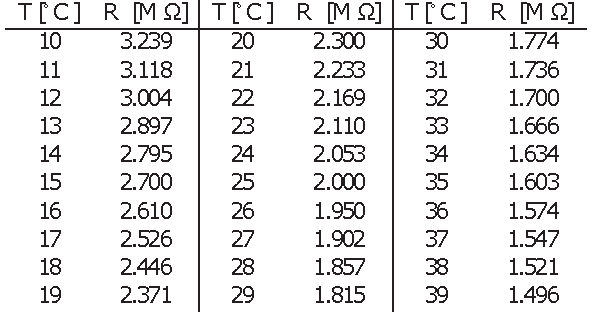
\includegraphics{figures/Temperatur.pdf}
  \caption{Temperatur der Luft bei verschiedenen Widerständen \cite{ap12}\, .} 
  \label{fig:abb3}
\end{figure}
Die Viskosität von Luft kann durch die \autoref{fig:viskositaet} bestimmt werden.
\begin{figure}[H]
  \centering
  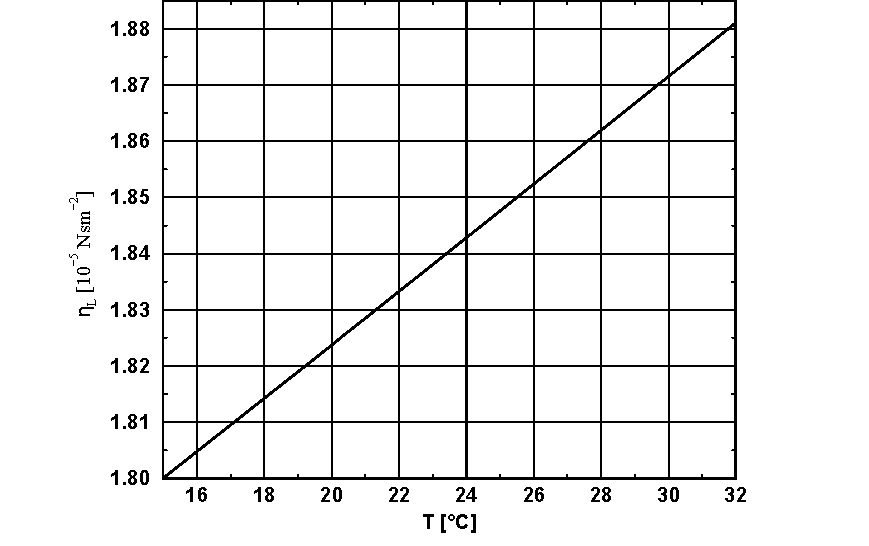
\includegraphics{figures/Viskositaet.pdf}
  \caption{Die Viskosität von Luft bei verschiedenen Temperaturen  \cite{ap12}\, .} 
  \label{fig:viskositaet}
\end{figure}


Um die Ladung der Öltröpfchen zu ermitteln, wurden Messungen bei fünf verschiedenen Spannungen für jeweils fünf Tröpfchen durchgeführt.
Alle Zeiten wurden für eine Strecke von $s = 0,5 \, \unit{\milli\meter}$ gemessen.
Die Widerstände können aufgrund der Genauigkeit des Geräts nur auf zwei Nachkommastellen abgelesen werden, zur Temperaturermittlung
müssen also entsprechende Rundungen getroffen werden. \\

Dabei übersetzen sich die gemessenen Widerstände wie folgt in Temperaturen und Viskositäten:
\begin{align*}
  R &= 1,99 \,\si{\mega\ohm} \Leftrightarrow T = 25 \,\si{\celsius} \Leftrightarrow \eta_\text{L} = 1,8475 \cdot 10^{-5} \,\unit{\newton} \unit{\dfrac{\second}{\meter^2}} \Leftrightarrow R = 1,98 \, \si{\mega\ohm} \\
  R &= 1,97 \,\si{\mega\ohm} \Leftrightarrow T = 26 \,\si{\celsius} \Leftrightarrow \eta_\text{L} = 1,8525 \cdot 10^{-5} \,\unit{\newton} \unit{\dfrac{\second}{\meter^2}} \,.
\end{align*}
Für alle aufgenommen Zeiten sei im Folgenden ein menschlicher Messfehler von $200 \,\si{\milli\second}$ angesetzt, die Spannungen sind auf $\pm 2 \,\si{\volt}$ genau angegeben.
\begin{table}[H]
    \caption{Messdaten der Öltröpfchen für verschiedene Spannungen $U$.}
    \label{tab:t_werte}
        \begin{tabular}{c c c c c}
            \begin{tabular}{S S[table-format=1.3] S[table-format=1.3]}
              %\caption{Messdaten bei $R = 1,99 \,\si{\mega\ohm}$, $U = 157 \,\si{\volt}$.}
              \toprule
              {Teilchen} & {$ t_{ab} \mathbin{/} \unit{\second}$} & {$ t_{auf} \mathbin{/} \unit{\second}$}\\
              \midrule
              1                                &     6.690     &     3.612       \\
              {($U = 157 \,\si{\volt}$)}       &     3.422     &     6.297       \\
                                               &     7.938     &     5.690       \\
              2                                &     4.04      &     4.44        \\
                                               &     4.97      &     4.20        \\
                                               &     4.53      &     4.71        \\
              3                                &     4.44      &     5.98        \\
                                               &     4.32      &     5.43        \\
                                               &     4.15      &     5.34        \\
              4                                &     4.85      &     5.64        \\
                                               &     9.31      &     8.49        \\
                                               &     7.02      &     8.75        \\
              5                                &     3.86      &     4.37        \\
                                               &     3.85      &     4.11        \\
                                               &     3.75      &     4.35        \\
              \bottomrule
            \end{tabular}
            \begin{tabular}{S S[table-format=1.3] S[table-format=1.2]}
              %\caption{Messdaten bei $R = 1,99 \,\si{\mega\ohm}$, $U = 175 \,\si{\volt}$.}
              \toprule
              {Teilchen}&{$ t_{ab} \mathbin{/} \unit{\second}$} & {$ t_{auf} \mathbin{/} \unit{\second}$}\\
              \midrule
              6                                 &     3.73      &      3.02     \\
              {($U = 175 \,\si{\volt}$)}        &     4.20      &      3.23     \\
                                                &     4.63      &      3.47     \\
              7                                 &     3.43      &      4.13     \\
                                                &     3.08      &      4.42     \\
                                                &     3.52      &      4.11     \\
              8                                 &     3.12      &      3.03     \\
                                                &     3.30      &      3.85     \\
                                                &     2.49      &      2.77     \\
              9                                 &     3.06      &      2.85     \\
                                                &     2.86      &      3.23     \\
                                                &     3.20      &      2.97     \\
              10                                &     2.09      &      2.14     \\
                                                &     2.21      &      2.51     \\
                                                &     2.43      &      1.98     \\
              \bottomrule
            \end{tabular}
            \begin{tabular}{S S[table-format=1.3] S[table-format=1.2]}
              %\caption{Messdaten bei $R = 1,98 \,\si{\mega\ohm}$, $U = 200 \,\si{\volt}$.}
              \toprule
              {Teilchen}&{$ t_{ab} \mathbin{/} \unit{\second}$} & {$ t_{auf} \mathbin{/} \unit{\second}$}\\
              \midrule
              11                                &      3.32     &      3.43      \\
              {($U = 200 \,\si{\volt}$)}        &      3.86     &      3.92      \\
                                                &      3.61     &      3.24      \\
              12                                &      3.52     &      3.82      \\
                                                &      3.90     &      3.85      \\
                                                &      3.63     &      3.85      \\
              13                                &      2.75     &      2.67      \\
                                                &      2.02     &      2.36      \\
                                                &      2.44     &      2.54      \\
              14                                &      4.54     &      5.10      \\
                                                &      4.40     &      4.90      \\
                                                &      4.47     &      4.77      \\
              15                                &      2.30     &      1.67      \\
                                                &      1.90     &      2.10      \\
                                                &      2.05     &      2.11      \\
              \bottomrule
            \end{tabular} \\
            \\
            \begin{tabular}{S S[table-format=1.3] S[table-format=1.2]}
              %\caption{Messdaten bei $R = 1,98 \,\si{\mega\ohm}$, $U = 225 \,\si{\volt}$.}
              \toprule
              {Teilchen}&{$ t_{ab} \mathbin{/} \unit{\second}$} & {$ t_{auf} \mathbin{/} \unit{\second}$}\\
              \midrule
                16                                &     1.89      &      1.96     \\
                {($U = 225 \,\si{\volt}$)}        &     1.88      &      1.95     \\
                                                  &     2.05      &      1.75     \\
                17                                &     1.33      &      1.37     \\
                                                  &     1.97      &      2.05     \\
                                                  &     1.49      &      1.38     \\
                18                                &     2.94      &      3.39     \\
                                                  &     3.13      &      3.37     \\
                                                  &     3.14      &      3.29     \\
                19                                &     3.19      &      3.10     \\
                                                  &     2.99      &      3.56     \\
                                                  &     3.15      &      3.07     \\
                20                                &     2.93      &      2.88     \\
                                                  &     2.70      &      2.95     \\
                                                  &     2.73      &      3.00     \\
              \bottomrule
            \end{tabular} 
            \begin{tabular}{S S[table-format=1.3] S[table-format=1.2]}
              %\caption{Messdaten bei $R = 1,97 \,\si{\mega\ohm}$, $U = 250 \,\si{\volt}$.}
              \toprule
              {Teilchen}&{$ t_{ab} \mathbin{/} \unit{\second}$} & {$ t_{auf} \mathbin{/} \unit{\second}$}\\
              \midrule
                21                                &     2.04      &      2.27     \\
                {($U = 250 \,\si{\volt}$)}        &     2.15      &      2.12     \\
                                                  &     2.08      &      2.06     \\
                22                                &     2.29      &      2.33     \\
                                                  &     2.08      &      2.25     \\
                                                  &     1.98      &      2.36     \\
                23                                &     4.12      &      4.29     \\
                                                  &     3.23      &      3.90     \\
                                                  &     4.02      &      4.33     \\
                24                                &     3.13      &      3.26     \\
                                                  &     2.80      &      3.51     \\
                                                  &     3.09      &      3.29     \\
                25                                &     2.27      &      2.63     \\
                                                  &     2.67      &      2.93     \\
                                                  &     3.03      &      3.04     \\
              \bottomrule
            \end{tabular}
          \end{tabular}
\end{table}
Mit dem Zeit-Weg-Gesetz
\begin{equation*}
  v = \dfrac{s}{t}
\end{equation*}
wird die Geschwindigkeit der von jedem einzelnen Tröpfchen bestimmt. \\
Die berechneten Geschwindigkeiten sind in \autoref{tab:geschw} aufgetragen.
\begin{table}[H]
  \caption{Geschwindigkeiten der Öltröpfchen für verschiedene Spannungen}
  \label{tab:geschw}
  \centering
  \begin{subtable}[t]{0.45\textwidth}
      \small
      \subcaption{Daten für $U=\qty{157}{\volt}$}
      \label{stab:v157}
      \begin{table}[H]
          \centering
          \begin{tabular}{S S S}
            \toprule
              {Nr}& {$ v_\text{auf} \mathbin{/} \dfrac{\unit{\milli\meter}}{\unit{\second}}$}&{$ v_\text{ab} \mathbin{/} \dfrac{\unit{\milli\meter}}{\unit{\second}}$}\\
            \midrule
              1     &     {$0,1019 \pm 0,0029$}     &     {$0,0946 \pm 0,0030$}        \\
              2     &     {$0,1126 \pm 0,0029$}     &     {$0,1116 \pm 0,0029$}        \\
              3     &     {$0,0898 \pm 0,0019$}     &     {$0,1163 \pm 0,0031$}        \\
              4     &     {$0,0682 \pm 0,0012$}     &     {$0,0760 \pm 0,0016$}        \\
              5     &     {$0,1170 \pm 0,0032$}     &     {$0,1310 \pm 0,0040$}        \\
            \bottomrule
          \end{tabular}
        \end{table}
      
  \end{subtable}\qquad
  \begin{subtable}[t]{0.45\textwidth}
      \small
      \subcaption{Daten für $U=\qty{175}{\volt}$}
      \label{stab:v175}
      \begin{table}[H]
          \centering
          \begin{tabular}{S S S}
            \toprule
            {Nr}& {$ v_\text{auf} \mathbin{/} \dfrac{\unit{\milli\meter}}{\unit{\second}}$}&{$ v_\text{ab} \mathbin{/} \dfrac{\unit{\milli\meter}}{\unit{\second}}$}\\
            \midrule
             6      &   	  {$0,155 \pm 0,006$}     &     {$0,120 \pm 0,003$}       \\
             7      &   	  {$0,119 \pm 0,003$}     &     {$0,150 \pm 0,005$}       \\
             8      &   	  {$0,158 \pm 0,006$}     &     {$0,171 \pm 0,007$}       \\
             9      &   	  {$0,166 \pm 0,006$}     &     {$0,165 \pm 0,006$}       \\
            10      &   	  {$0,228 \pm 0,012$}     &     {$0,224 \pm 0,012$}       \\
            \bottomrule
          \end{tabular}
        \end{table}
      
  \end{subtable}\qquad
  \begin{subtable}[t]{0.45\textwidth}
      \small
      \subcaption{Daten für $U=\qty{200}{\volt}$}
      \label{stab:v200}
      \begin{table}[H]
          \centering
          \begin{tabular}{S S S}
            \toprule
            {Nr}& {$ v_\text{auf} \mathbin{/} \dfrac{\unit{\milli\meter}}{\unit{\second}}$}&{$ v_\text{ab} \mathbin{/} \dfrac{\unit{\milli\meter}}{\unit{\second}}$}\\
            \midrule
            11      &     {$0,143 \pm 0,005$}     &     {$0,140 \pm 0,005$}     \\
            12      &     {$0,130 \pm 0,004$}     &     {$0,136 \pm 0,004$}     \\
            13      &     {$0,199 \pm 0,009$}     &     {$0,211 \pm 0,011$}     \\
            14      &     {$0,102 \pm 0,002$}     &     {$0,112 \pm 0,003$}     \\
            15      &     {$0,258 \pm 0,016$}     &     {$0,241 \pm 0,014$}     \\
            \bottomrule
          \end{tabular}
        \end{table}
      
  \end{subtable}\qquad
  \begin{subtable}[t]{0.45\textwidth}
      \small
      \subcaption{Daten für $U=\qty{225}{\volt}$}
      \label{stab:v225}
      \begin{table}[H]
          \centering
          \begin{tabular}{S S S}
            \toprule
              {Nr}& {$ v_\text{auf} \mathbin{/} \dfrac{\unit{\milli\meter}}{\unit{\second}}$}&{$ v_\text{ab} \mathbin{/} \dfrac{\unit{\milli\meter}}{\unit{\second}}$}\\
            \midrule
            16      &     {$0,266 \pm 0,016$}     &     {$0,25 \pm 0,015$}     \\
            17      &     {$0,324 \pm 0,026$}     &     {$0,32 \pm 0,026$}     \\
            18      &     {$0,149 \pm 0,005$}     &     {$0,16 \pm 0,006$}     \\
            19      &     {$0,155 \pm 0,006$}     &     {$0,16 \pm 0,006$}     \\
            20      &     {$0,170 \pm 0,007$}     &     {$0,18 \pm 0,007$}     \\
            \bottomrule
          \end{tabular}
        \end{table}
      
  \end{subtable}\qquad
  
  \begin{subtable}[t]{0.45\textwidth}
      \small
      \subcaption{Daten für $U=\qty{250}{\volt}$}
      \label{stab:v250}
      \begin{table}[H]
          \centering
          \begin{tabular}{S S S}
            \toprule
              {Nr}& {$ v_\text{auf} \mathbin{/} \dfrac{\unit{\milli\meter}}{\unit{\second}}$}&{$ v_\text{ab} \mathbin{/} \dfrac{\unit{\milli\meter}}{\unit{\second}}$}\\
            \midrule
            21      &     {$0,233 \pm 0,013$}     &   	  {$0,239 \pm 0,013$}     \\
            22      &     {$0,216 \pm 0,011$}     &   	  {$0,236 \pm 0,013$}     \\
            23      &     {$0,120 \pm 0,003$}     &   	  {$0,132 \pm 0,004$}     \\
            24      &     {$0,149 \pm 0,005$}     &   	  {$0,167 \pm 0,006$}     \\
            25      &     {$0,175 \pm 0,007$}     &   	  {$0,191 \pm 0,009$}     \\
            \bottomrule
          \end{tabular}
        \end{table}
  \end{subtable}
\end{table}

Um die Ladungen zu berechnen, muss zunächst die effektive Viskosität mit \eqref{eq:Veff}, der Radius der Tröpfchen mit \eqref{eq:rmitEfled} 
und die korrigierte Ladung mit \eqref{eq:qKorr} ermittelt werden.
Die berechneten Radien sind in \autoref{tab:radien}, die nicht korrigierten Ladungen in \autoref{tab:ladungennichtkorr}
und die korrigierten Ladungen in \autoref{tab:Ladungen} aufgetragen und mitsamt Fehlerbalken in \autoref{fig:ladungen} graphisch dargestellt.


\begin{table}[H]
  \centering
  \caption{Berechnete Radien $r$.}
  \label{tab:radien}
  \begin{tabular}{S S S S}
    \toprule
      {$\text{Nr}$} & {$r \mathbin{/} 10^{-7} \, \unit{\meter}$} & {$\text{Nr}$} & {$r \mathbin{/} 10^{-7} \, \unit{\meter}$}\\
    \midrule
     1      &      {$6,897 \pm 0,267$}      &      14      &      {$3,111 \pm 0,594$}     \\
     2      &      {$3,161 \pm 0,707$}      &      15      &      {$5,448 \pm 2,450$}     \\
     3      &      {$5,035 \pm 0,349$}      &      16      &      {$4,121 \pm 3,052$}     \\
     4      &      {$3,208 \pm 0,285$}      &      17      &      {$3,795 \pm 4,765$}     \\
     5      &      {$3,603 \pm 0,709$}      &      18      &      {$3,530 \pm 1,167$}     \\
     6      &      {$5,743 \pm 0,552$}      &      19      &      {$3,048 \pm 1,662$}     \\       
     7      &      {$5,384 \pm 0,566$}      &      20      &      {$3,179 \pm 1,886$}     \\
     8      &      {$3,700 \pm 1,406$}      &      21      &      {$2,720 \pm 4,615$}     \\
     9      &      {$3,727 \pm 1,183$}      &      22      &      {$4,108 \pm 2,646$}     \\
    10      &      {$4,699 \pm 2,441$}      &      23      &      {$3,376 \pm 0,831$}     \\
    11      &      {$2,474 \pm 1,509$}      &      24      &      {$3,813 \pm 1,227$}     \\
    12      &      {$2,426 \pm 1,426$}      &      25      &      {$3,367 \pm 3,556$}     \\
    13      &      {$3,639 \pm 2,056$}      &      {-}     &              {-}             \\
    \bottomrule
  \end{tabular}
\end{table}


\begin{table}[H]
  \centering
  \caption{Nicht korrigierte Ladungen $q$ für alle betrachtete Teilchen.}
  \label{tab:ladungennichtkorr}
  \begin{tabular}{S S S S}
    \toprule
      {$\text{Nr}$} & {$q \mathbin{/} 10^{-19} \, \unit{\coulomb}$} & {$\text{Nr}$} & {$q \mathbin{/} 10^{-19} \,\unit{\coulomb}$}\\
    \midrule
     1      &     {$6,373 \pm 0,407$}     &     14      &     {$2,214 \pm 0,486$}      \\
     2      &     {$3,230 \pm 0,773$}     &     15      &     {$9,208 \pm 4,337$}      \\
     3      &     {$4,714 \pm 0,398$}     &     16      &     {$6,607 \pm 5,188$}      \\
     4      &     {$2,176 \pm 0,243$}     &     17      &     {$7,597 \pm 1,.76$}      \\
     5      &     {$4,057 \pm 0,868$}     &     18      &     {$3,372 \pm 1,229$}      \\
     6      &     {$6,605 \pm 0,793$}     &     19      &     {$2,912 \pm 1,744$}      \\
     7      &     {$6,080 \pm 0,763$}     &     20      &     {$3,403 \pm 2,149$}      \\
     8      &     {$5,106 \pm 2,131$}     &     21      &     {$3,493 \pm 6,426$}      \\
     9      &     {$5,165 \pm 1,766$}     &     22      &     {$5,159 \pm 3,469$}      \\
    10      &     {$8,833 \pm 5,043$}     &     23      &     {$2,411 \pm 0,692$}      \\
    11      &     {$2,372 \pm 1,506$}     &     24      &     {$3,311 \pm 1,214$}      \\
    12      &     {$2,172 \pm 1,347$}     &     25      &     {$3,536 \pm 3,509$}      \\
    13      &     {$5,168 \pm 2,956$}     &     {-}     &               {-}                \\
    \bottomrule
  \end{tabular}
\end{table}

\begin{table}[H]
  \centering
  \caption{Korrigierte Ladungen $q_0$ für alle betrachteten Teilchen.}
  \label{tab:Ladungen}
  \begin{tabular}{S S S S}
    \toprule
      {$\text{Nr}$} & {$q_0 \mathbin{/} 10^{-19} \, \unit{\coulomb}$} & {$\text{Nr}$} & {$q_0 \mathbin{/} 10^{-19} \,\unit{\coulomb}$}\\
    \midrule
         1      &       {$6,864 \pm 0,421$}     &     14      &       {$2.584 \pm 5,030$} \\
         2      &       {$3,762 \pm 0,787$}     &     15      &       {$10.10 \pm 4,372$} \\
         3      &       {$5,208 \pm 0,408$}     &     16      &       {$7.448 \pm 5,249$} \\
         4      &       {$2,530 \pm 0,254$}     &     17      &       {$8.645 \pm 10,99$} \\
         5      &       {$4,645 \pm 0,883$}     &     18      &       {$3.872 \pm 1,257$} \\
         6      &       {$7,214 \pm 0,813$}     &     19      &       {$3.408 \pm 1,785$} \\
         7      &       {$6,677 \pm 0,780$}     &     20      &       {$3.960 \pm 2,186$} \\
         8      &       {$5,828 \pm 2,169$}     &     21      &       {$4.157 \pm 6,569$} \\
         9      &       {$5,890 \pm 1,793$}     &     22      &       {$5.818 \pm 3,509$} \\
        10      &       {$9,823 \pm 5,109$}     &     23      &       {$2.784 \pm 0,722$} \\
        11      &       {$2,866 \pm 1,534$}     &     24      &       {$3.766 \pm 1,250$} \\
        12      &       {$2,634 \pm 1,376$}     &     25      &       {$4.084 \pm 3,500$} \\
        13      &       {$5,911 \pm 2,981$}     &     {-}     &             {-}           \\
    \bottomrule
  \end{tabular}
\end{table}


\begin{figure}
  \centering
  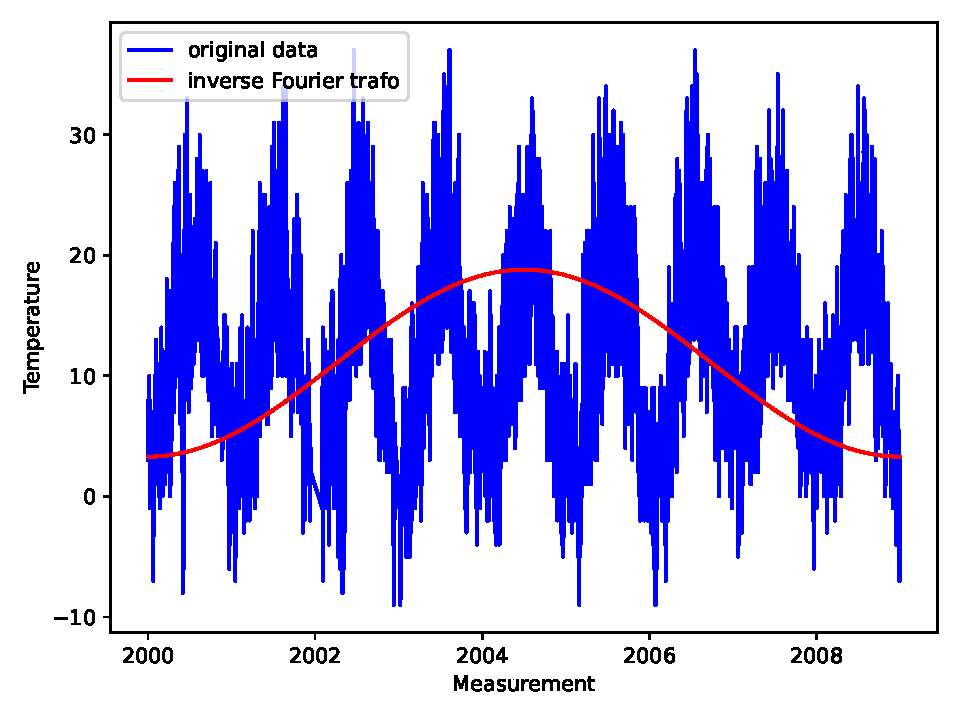
\includegraphics{build/e.pdf}
  \caption{Berechnete Ladungen $q$ mit Fehlerbalken.}
  \label{fig:ladungen}
\end{figure}

Es ist unrealistisch, dass alle Ladungen einem ganzzahliges Vielfachen von eines einzelnen Wertes entsprechen, also wird der kleinste gemeinsame Teiler gesucht, bei dem die übrigbleibende Differenz unter $1 \cdot 10^{-19}$ liegt, da die Elementarladung in dieser Größenordnung vermutet wird.
Mit dieser Methode wird eine Ladung von
\begin{equation*}
  e_{0,\text{unkorr}} = \qty{4.61(0.78)e-19} \,\si{\coulomb}
\end{equation*} 
ohne und
\begin{equation*}
  e_{0,\text{korr}} = \qty{5.2(0.8)e-19} \,\unit{\coulomb}
\end{equation*}
mit Korrektur berechnet. \\

Daraus kann über die Faraday-Konstante $ F = 96485,33212... \dfrac{\unit{\coulomb}}{\text{mol}}$ \cite{go02} mit der Gleichung 
\begin{equation*}
  N_\text{A} = \dfrac{F}{e_0}
\end{equation*}
die Avogadro-Konstante bestimmt werden, welche 
sich zu
\begin{equation*}
  N_\text{A, unkorr} = \qty{2.09(0.35)e+23} \,\dfrac{1}{\si{\mol}}
\end{equation*}
ohne und
\begin{equation*}
  N_\text{A, korr} = \qty{1.85(0.29)e23} \, \dfrac{1}{\si{mol}}
\end{equation*}
mit Korrektur ergibt.